\begin{intersong}
	\begin{center}
		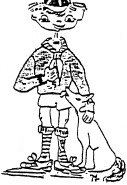
\includegraphics[width=0.2\textwidth]{kijkdateensaan}
	\end{center}
\end{intersong}
\beginsong{Kijk dat eens aan}
\beginverse*
Kijk dat eens aan \rep{2}
Wat wilde troep \rep{2}
Wat hels lawaai \rep{2}
Wat dom geroep\rep{2}
\endverse
\beginchorus
Bij 't zien van zo’n kerels,
maakt U maar geen verdriet,
twee maanden bij de wolfjes,
en jij herkent ze niet.
\endchorus
\beginverse*
Ze lopen scheef \rep{2}
Ze staan niet fiks \rep{2}
Van rij of rang \rep{2}
Verstaan ze niets \rep{2}
\endverse
\beginverse*
Ze vinden niet \rep{2}
Een simpel spoor \rep{2}
langs pijl en kruis \rep{2}
Lopen ze door \rep{2}
\endverse
\beginverse*
Van fluit en mes \rep{2}
Van koord en staf \rep{2}
Weten ze niks \rep{2}
Volstrekt niks af \rep{2}
\endverse
\beginverse*
Ze weten niks \rep{2}
Van wet of groet \rep{2}
Van tweedeklas \rep{2}
Of tenderfoot \rep{2}
\endverse
\beginverse*
De knopen zijn \rep{2}
Hun onbekend \rep{2}
Ze kwamen nooit \rep{2}
In ene tent \rep{2}
\endverse
\beginverse*
Ze zijn zo dom \rep{2}
Zo vuil en wreed \rep{2}
En in een woord \rep{2}
Tot niks gereed \rep{2}
\endverse
\endsong